\subsection{Transaction Execution}
The transaction execution is the mechanism through which the world state is
updated. It represents a transition from one
valid state to another valid state.

\begin{figure}
	\begin{center}
		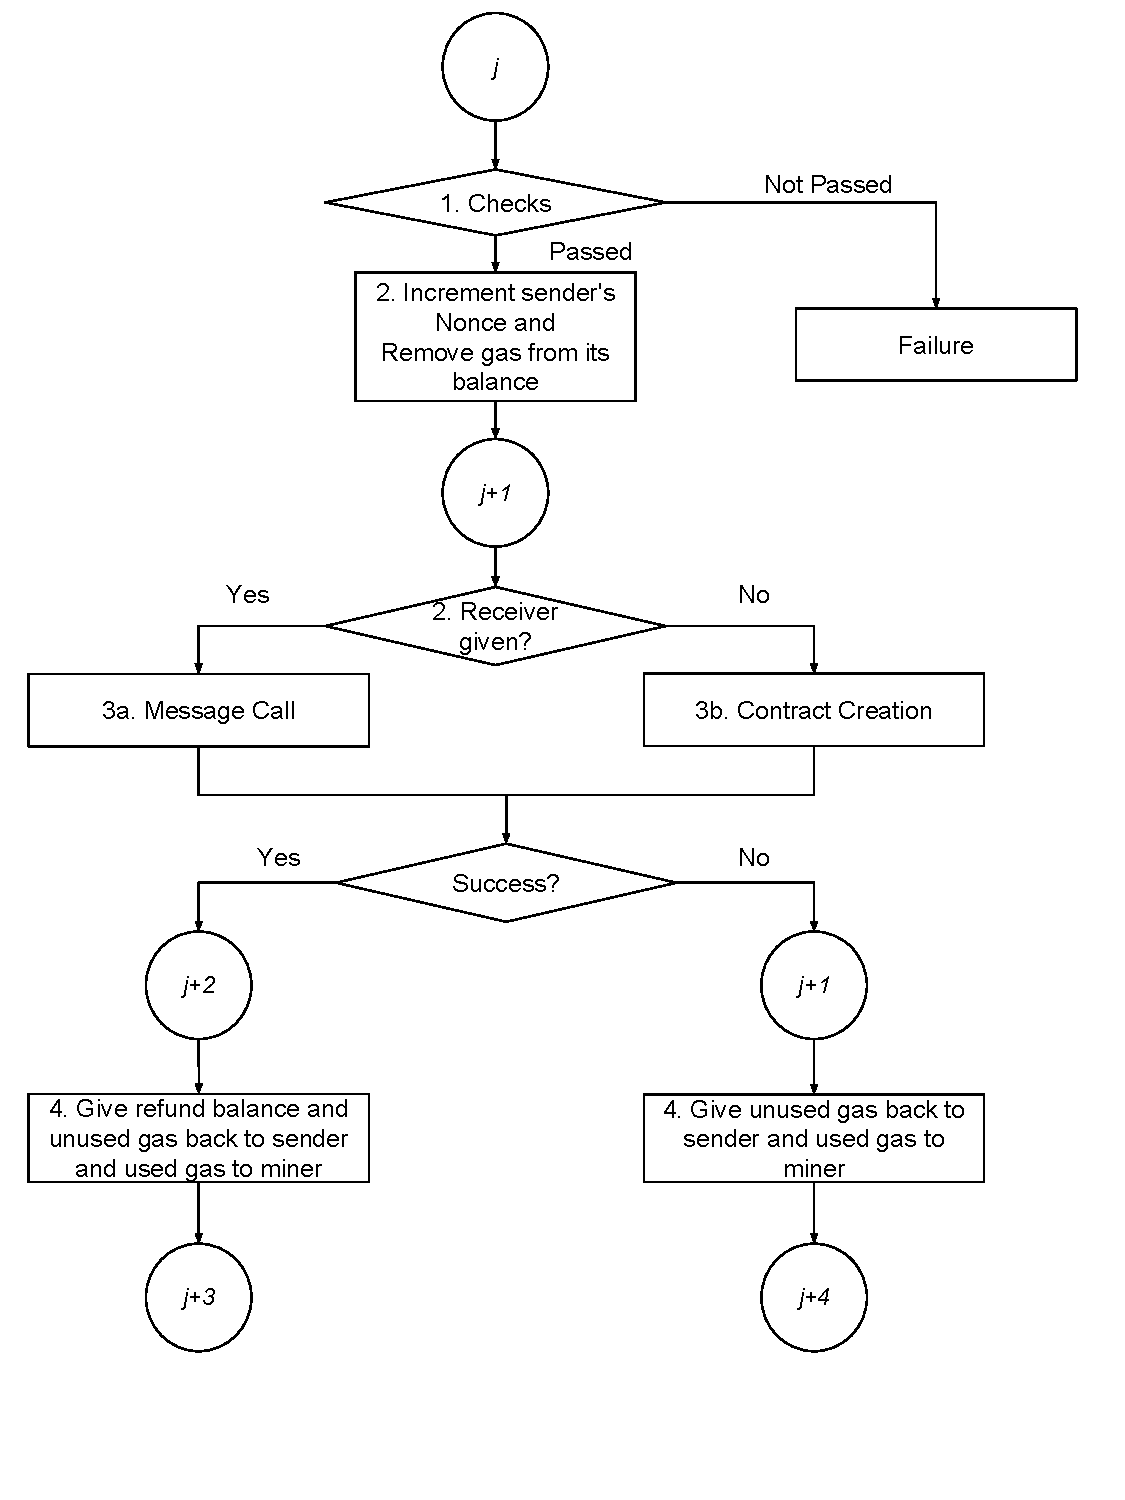
\includegraphics[width=\textwidth]{./res/img/transaction-execution.pdf}
	\end{center}
	\caption{The steps of the transaction execution algorithm.}
	\label{fig:tx:execution}
\end{figure}

\autoref{fig:tx:execution} summarizes the steps of the algorithm for the 
transaction execution:
\begin{enumerate}
	\item The transaction has to pass some simple validity checks, e.g.\ the
	transaction should be a well-formed RLP encoded string and the initiator
	of the transaction should have a balance big enough to afford the 
	transaction.
	Moreover, since a transaction should be included in a block and the block
	has in turn its own gas limit, it should be also true that the sum 
	of the accumulated gas used by the already included transactions and the gas
	limit of this transaction are smaller than the block's gas limit.
	If these checks fail, the transaction is simply not included in the block.
	
	
	\item The nonce of the initiator of the transaction is incremented by one and its balance is reduced by the product of the gas limit and the gas price. This modification to the state is irreversible.
	\item Now, depending on whether the receiver address is given or not
	we should make a distinction between:
	\begin{enumerate}[label=\alph*.]
		\item Message Calls (\autoref{sec:message-call}) and;
		\item Contract Creation (\autoref{sec:contract-creation}).
	\end{enumerate}
	During the execution of the message call or contract creation the system
	keeps track of the \textbf{transaction substate}, i.e.\ some important
	information that are later used to complete the state transition.
	The transaction substate includes the \textbf{touched accounts}, the set of
	accounts that will be discarded following the completion 
	(\textbf{self-destruct set}) and the
	\textbf{refund balance}, that is an amount of gas that is incremented by
	removing elements from the world state, e.g. by setting a non-zero value to
	a zero value in the storage or by removing a contract from the state.
	
	\item Once the message call or the contract creation are concluded
	the sum of the remaining gas and the refund balance are refund
	to the initiator of the transaction at the transaction's gas price~\footnote{This sum cannot exceed the initial allocated
	price~\cite{wood2018ethereum}, in other words the refund balance can be 
	used to mitigate the transaction cost, but not to profit.}.
	If the message call or contract creation did not complete successfully,
	their state is reverted and the refund balance is zeroed, since its
	modifications to the state are not considered.
	The gas used is given to the beneficiary address (i.e. the miner), who
	built and finalized the block. Finally, the self-destruct set and the
	touched accounts that became empty or dead after the transaction should
	be deleted from the world  state.
\end{enumerate}
 

